\documentclass{YourPres}

% aux colors -- examples
\def \xColor {\color{red}}
\def \yColor {\color{YourBase}}

% info for titlepage
\title{Пример использования стилевого шаблона презентации в~\XeLaTeX}
\author{Валерия Пузикова}

\begin{document}
  \Yourtitlepage

  \begin{frame}{Пояснения}
    \begin{itemize}
      \item[\YourCheckedbox] Эта презентация создана в \LaTeX{} (точнее, в \XeLaTeX{}).\\
      \item[\YourCheckedbox] Стиль и некоторые полезные команды определены в файле YourPres.cls.\\
      \item[\YourCrossedbox] Использование \LaTeX{} для презентаций сильно облегчает
         \begin{itemize}
            \item перенос в презентацию сложных <<многоэтажных>> формул и алгоритмов из научных статей, сверстанных в \LaTeX{}; \\
            \item вставку в презентацию листингов кода с автоматическим сохранением подсветки синтаксиса для широкого спектра языков программирования (и ее стилизацией под выбранную палитру).\\
         \end{itemize}
      \item[\YourHandRight] Для компиляции презентации необходимо использовать \XeLaTeX{} $\Rightarrow$ PDF, поскольку установленные шрифты не сконвертированы в \TeX{} формат.\\
      \item[\YourHandRight] Исходный файл с текстом презентации должен быть \textbf{строго} в кодировке UTF8 для корректной компиляции \XeLaTeX{} $\Rightarrow$ PDF!\\
      \item[\YourHandRight] Для встраивания в презентацию видео или анимаций их необходимо предварительно разбить на последовательность изображений-кадров (например, при помощи своего скрипта/онлайн-конвертера/...). Встраивание последовательности изображений при помощи {\Yourcode\textbackslash animategraphics} позволяет получить презентацию с анимациями, проигрывающимися в любых версиях Adobe Acrobat (с~конца 2020~года Flash Player не поддерживается).
    \end{itemize}
  \end{frame}


  \section{Инженерный контент}

  \begin{frame}[fragile]{Вставка листингов кода}\vspace*{-0.25cm}
    \begin{minipage}[h]{0.7\linewidth}
      \begin{lstlisting}[language=C++,style=CUDA,label=lst1,caption=CUDA Samples -- 5]
// calculate grid hash value for each particle
__global__
void calcHashD(uint   *gridParticleHash,  // output
               uint   *gridParticleIndex, // output
               float4 *pos,               // input: positions
               uint    numParticles)
{
    uint index = __umul24(blockIdx.x, blockDim.x) + threadIdx.x;

    if (index >= numParticles) return;

    volatile float4 p = pos[index];

    // get address in grid
    int3 gridPos = calcGridPos(make_float3(p.x, p.y, p.z));
    uint hash = calcGridHash(gridPos);

    // store grid hash and particle index
    gridParticleHash[index] = hash;
    gridParticleIndex[index] = index;
}
      \end{lstlisting}
    \end{minipage}\hspace*{0.3cm}
    \begin{minipage}[h]{0.27\linewidth}\vskip4pt
       \lstinputlisting[language=Python, linerange={2-4,6-13,32-35},title=Вставка из example.py]{code/example.py}
    \end{minipage}
  \end{frame}

  \begin{frame}{Вставка рисунков; верстка формул и алгоритмов}
    \begin{minipage}[h]{0.38\linewidth}
      \begin{center}
         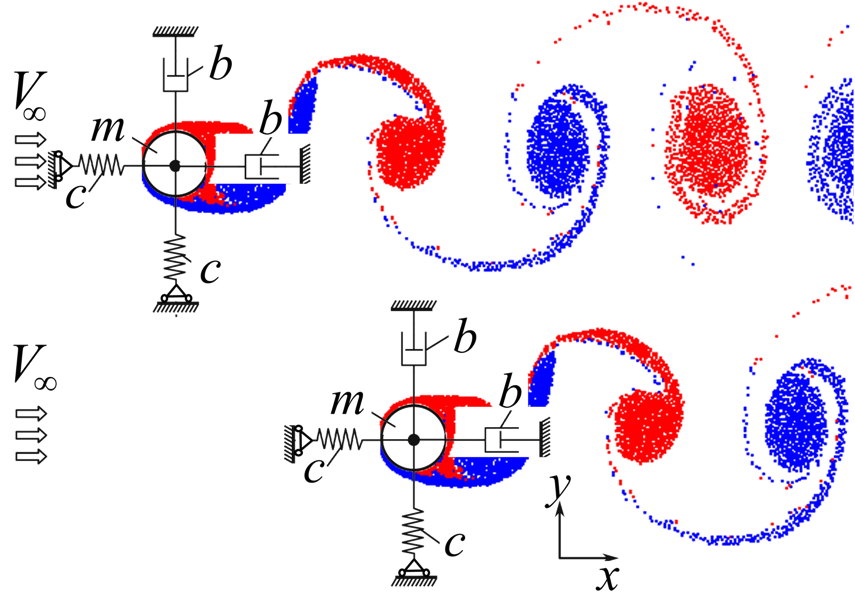
\includegraphics[width=0.6\linewidth]{img/model.png}
         \captionof{figure}{Верхний рисунок с подрисуночной подписью, нижний без нее}\vskip20pt
         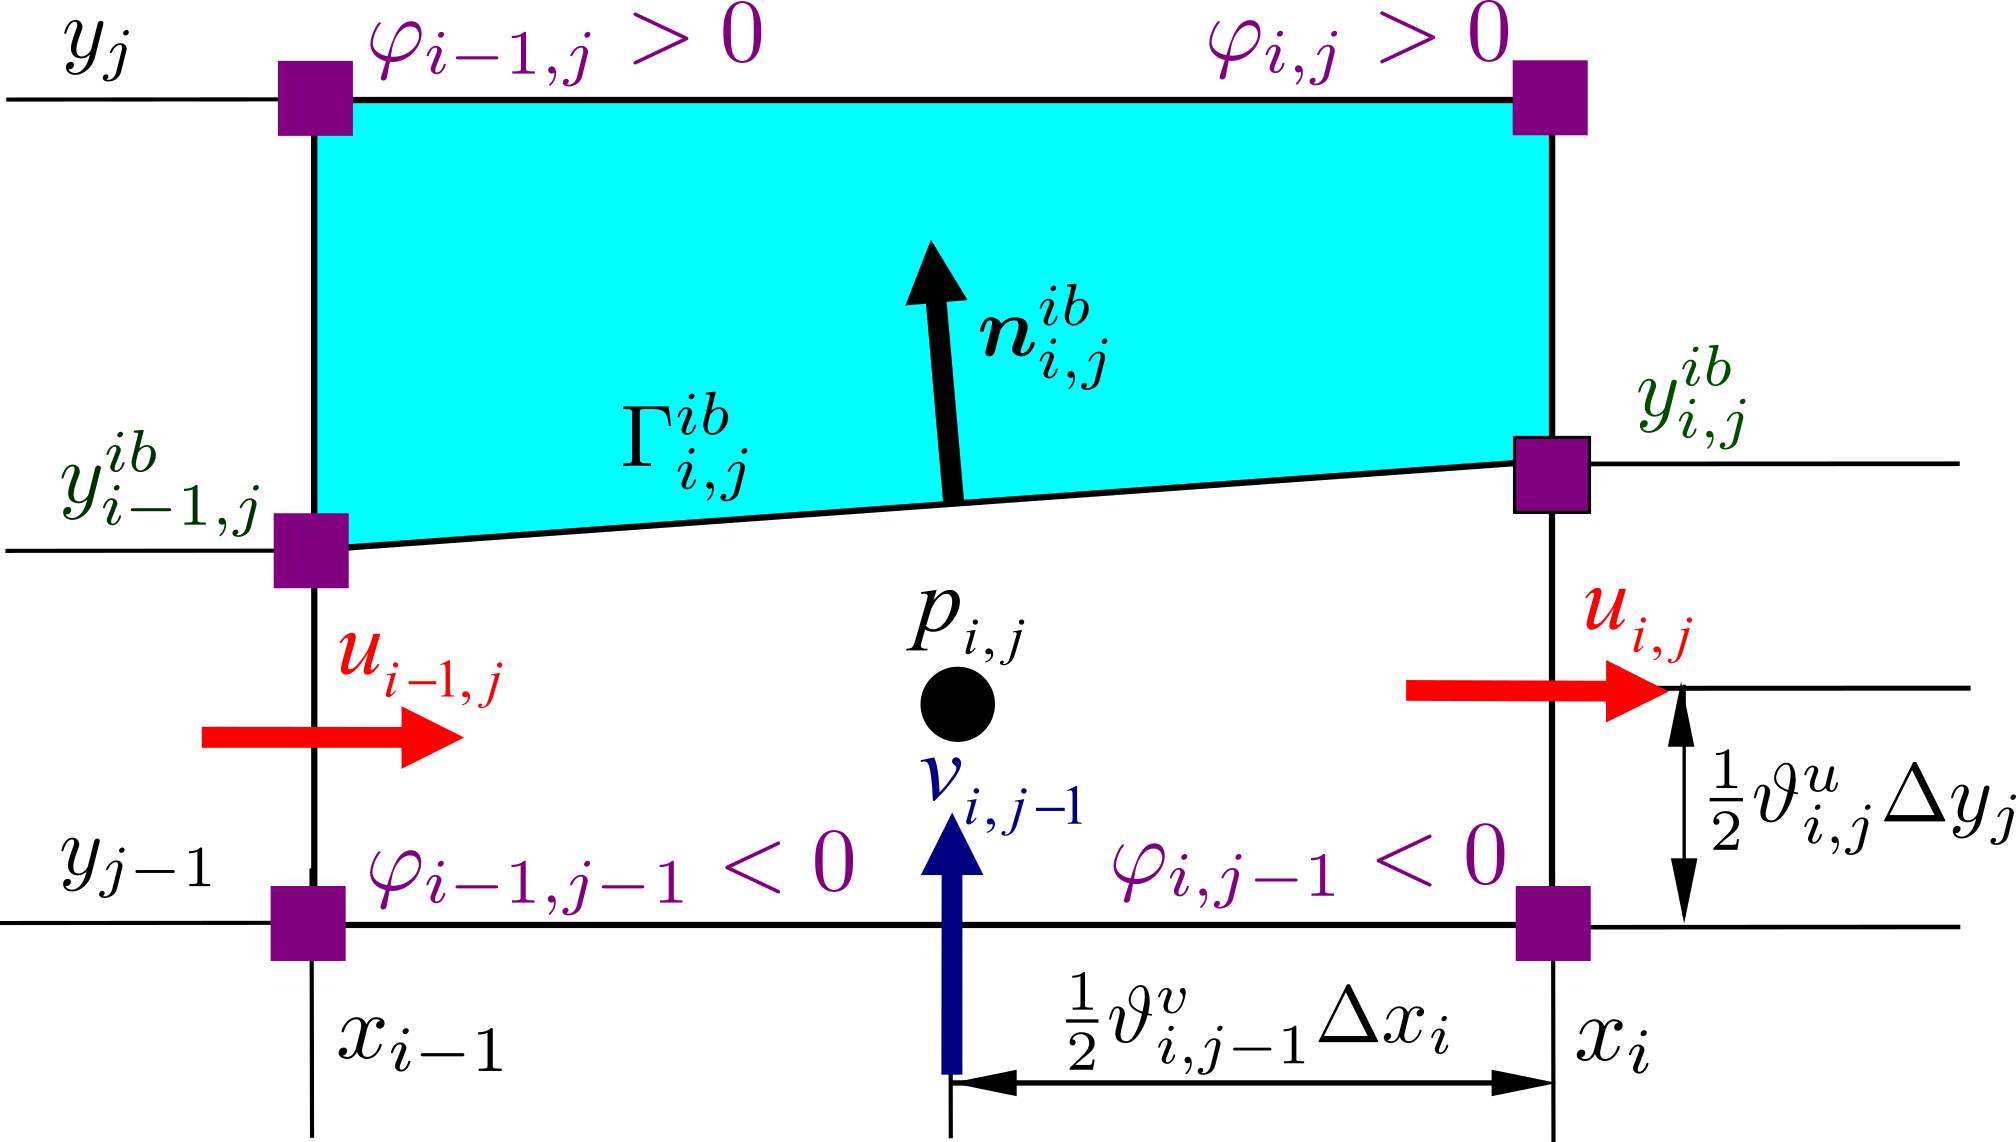
\includegraphics[width=0.9\linewidth]{img/cut_cell.png}
      \end{center}
    \end{minipage}\hfill
    \begin{minipage}[h]{0.6\linewidth}\vskip-3pt
      \begin{block}{После перенумерации КО $Ax=b$ примет вид: }
        \centering{
           $\begin{bmatrix}
              A_{0, 0} & \Theta & \dots & \Theta & {\color{YourBase}A_{0, s}} \\
              \vdots & \vdots & \ddots & \vdots & \vdots \\
              \Theta & \Theta  & \dots & A_{P - 1, P - 1} & {\color{YourBase}A_{P - 1, s} }\\
              {\color{YourParam2}A_{s, 0}} & {\color{YourParam2}A_{s, 1}} & \dots & {\color{YourParam2}A_{s, P - 1}} & {\color{YourBad}A_{s,s}}
           \end{bmatrix} \cdot \begin{bmatrix} x_0 \\ \vdots \\ x_{P - 1} \\ {\color{YourBad}x_s} \end{bmatrix}
          = \begin{bmatrix} b_0  \\ \vdots \\ b_{P - 1} \\ {\color{YourBad}b_s} \end{bmatrix}
          $}
      \end{block}\vskip-7pt
      \uncover<2> {
        \begin{minipage}[h]{0.47\linewidth}
          \begin{block}{Решение СЛАУ $Ax=b${\color{YourBase}р $\tilde{A}$}}
            \begin{algorithmic}[1]
  \For{$p = \overline{0, P - 1}$}
    \State{} $A_{p, p} t = b_p$\;
    \State{} ${\color{YourGood}\tilde{b}_s^p} ={\color{YourParam2} A_{s, p}} t$;
  \EndFor
  \State{} ${\color{YourGood}\tilde{A}_{s, s}} {\color{YourBad}x_s} = {\color{YourBad}b_s} - \sum\limits_{p = 0}^{P - 1} {\color{YourGood}\tilde{b}_s^p}$\;
  \For{$p = \overline{0, P - 1}$}
    \State{} $A_{p, p} x_p = b_p - {\color{YourBase}A_{p, s}} {\color{YourBad}x_s};$
  \EndFor
           \end{algorithmic}
         \end{block}
      \end{minipage}\hspace*{0.45cm}
      \begin{minipage}[h]{0.47\linewidth}
         \begin{block}{Расчет матрицы $\tilde{A}_{s, s}$}
            \begin{algorithmic}[1]
\For{$p = \overline{0, P - 1}$}
  \For{$c = \overline{0, N - 1}$}
    \State{} $A_{p, p} t = \left[ {\color{YourBase}A_{p, s}} \right]_c$\;
    \State{} $\left[ {\color{YourGood}\tilde{A}_{s, s}^p }\right]_c = {\color{YourParam2}A_{s, p}} t$\;
  \EndFor
\EndFor
\State{} ${\color{YourGood}\tilde{A}_{s, s}} =  {\color{YourBad}A_{s, s}} - \sum\limits_{p = 0}^{P - 1} {\color{YourGood}\tilde{A}_{s, s}^p}$.
            \end{algorithmic}\vskip2pt\mbox{ }
          \end{block}
       \end{minipage}
     }
    \end{minipage}
  \end{frame}

  \begin{frame}{Верстка таблиц}\vspace*{-0.3cm}
    \begin{block}{Для автостилизации таблиц необходимо}
      \begin{enumerate}
         \item Перед окружением таблицы использовать команду {\Yourcode\textbackslash Yourtable}, а, в случае таблиц, шапка которых состоит из четного числа строк, команду {\Yourcode\textbackslash Yourtable[evenheadrows]}.
         \item В преамбуле таблицы перед типом первого столбца поставить символ \Yourcolorbox{{\Yourcode =}}, а перед типами остальных столбцов -- \Yourcolorbox{{\Yourcode+}}, например: {\Yourcode \textbackslash begin\{tabular\}\{=c|+c|+c\}}.
         \item Перед каждой строкой шапки таблицы использовать команду {\Yourcode\textbackslash YourTableHeadRow}.
      \end{enumerate}
    \end{block}\vspace*{0.35cm}\\
    \begin{minipage}[t]{0.48\linewidth}
      \Yourtable
      \begin{tabularx}{\linewidth}{=X|+X|+X|+X}
         \YourTableHeadRow
Сетка & $ND$ & $N \times M$ & $\Delta t$\\
$G_1$ & 16 & $120 \times 148$ & \num{1e-2} \\
$G_2$ & 32 & $240 \times 296$ & \num{5e-3} \\
$G_3$ & 64 & $480 \times 592$ & \num{1e-3} \\
$G_4$ & 128 & $960 \times 1184$ & \num{5e-4}
      \end{tabularx}
   \end{minipage}\hspace*{0.2cm}
   \begin{minipage}[t]{0.51\linewidth}\vspace{-1.5cm}
      \begin{flushright}
         \Yourtable[evenheadrows]
         \begin{tabular}{=c|+c|+c}
            \YourTableHeadRow
 & \multicolumn{2}{+c}{Число итераций} \\
             \YourTableHeadRow
\multirow{-2}{*}{Уравнение}& Без DDM & С DDM \\
{\color{YourGood}Гельмгольца} & 2 & 1 \\
{\color{YourBad}Пуассона} & 8--12 & 1--2
         \end{tabular}
      \end{flushright}
    \end{minipage}
  \end{frame}

  \section{Графика}

  \begin{frame}{Палитра}\vspace*{-0.1cm}
    \begin{itemize}
      \item В таблице ниже собраны цвета, которые следует использовать для оформления графиков, диаграмм и пр. \\
      \item Цвета подложек блоков, строк таблиц, сносок, подписей и пр. уже указаны в стилевом файле --- в~файле презентации их задавать не требуется (и в таблице они не перечислены).
    \end{itemize}
    \vspace{0.1cm}
    \begin{center}
      \Yourtable
      \begin{tabular}{=c|+c|+l}
         \YourTableHeadRow
Цвет&Команда&Назначение\\  \hline
\fcolorbox{black}{YourBase}{{\color{white}\Yourcode 5B2C8C}} & {\Yourcode\textbackslash YourBase}& Основной параметр графика  \\ \hline
\fcolorbox{black}{YourParam}{{\color{white}\Yourcode AE2ADE}} & {\Yourcode\textbackslash YourParam}& Параметр графика  \\ \hline
\fcolorbox{black}{YourParam2}{{\color{white}\Yourcode 1AB2FB}} & {\Yourcode\textbackslash YourParam2}& Параметр 2 графика  \\ \hline
\fcolorbox{black}{YourParam3}{{\color{white}\Yourcode CEE832}} & {\Yourcode\textbackslash YourParam3}& Параметр 3 графика  \\ \hline
\fcolorbox{black}{YourParam4}{{\color{white}\Yourcode FFCA2B}} & {\Yourcode\textbackslash YourParam4}& Параметр 4 графика  \\ \hline
\fcolorbox{black}{YourAccent}{{\color{white}\Yourcode 605C61}} & {\Yourcode\textbackslash YourAccent}& Акцент\\ \hline
\fcolorbox{black}{YourBad}{{\color{white}\Yourcode D60020}} & {\Yourcode\textbackslash YourBad}& Состояние <<Плохо>>  \\ \hline
\fcolorbox{black}{YourNeutral}{{\color{white}\Yourcode FFCA2B}} & {\Yourcode\textbackslash YourNeutral}& Состояние <<Нейтрально>>  \\ \hline
\fcolorbox{black}{YourGood}{{\color{white}\Yourcode 00B27F}} & {\Yourcode\textbackslash YourGood}& Состояние <<Хорошо>>
       \end{tabular}
     \end{center}
  \end{frame}

  \begin{frame}{Встраивание анимаций}\vspace*{-0.5cm}
    \begin{minipage}[t]{0.54\linewidth}
      \begin{block}{Команды из YourPres.cls:}
      { \Yourcode
        \begin{itemize}
          \item  FramesAsGIF
          \item  FramesAsVideoPlayer
          \item  FramesAsVideoExtraPlayer
        \end{itemize}
      }
      \end{block}\vfill
      \begin{block}{Конвертация видео в png}
        свой скрипт/онлайн-конвертер/...
      \end{block}
    \end{minipage}\hfill
    \begin{minipage}[t]{0.4\linewidth}
      \begin{block}{Аргументы}
        \begin{enumerate}
          \item path to frames
          \item width
          \item height
          \item frame rate
          \item first frame number
          \item last frame number
        \end{enumerate}
      \end{block}\vspace{-0.2cm}
    \end{minipage}
    \mbox{ }\vspace{0.2cm}\\
    \FramesAsGIF{video/resonans/Re100Pair0_85Resonans-}{2.4cm}{2.4cm}{4}{0}{28}\hfill
    \FramesAsVideoPlayer{video/resonans/Re100Pair0_85Resonans-}{2.4cm}{2.4cm}{4}{0}{28}\hfill
    \FramesAsVideoExtraPlayer{video/resonans/Re100Pair0_85Resonans-}{2.4cm}{2.4cm}{4}{0}{28}\hspace{0.45cm}\mbox{ }
  \end{frame}

  \section{Иконки}

  \begin{frame}{Блоки с иконками}
    \begin{minipage}[h]{0.27\linewidth}
      \begin{block}[tools]{Блок с иконкой}
        Это обычное окружение {\Yourcode block}, но с опциональным аргументом --- названием иконки.
      \end{block}
    \end{minipage}\hfill
    \begin{minipage}[h]{0.27\linewidth}
      \begin{block}[filesystem2]{Банк иконок}
        Все иконки-примеры собраны в \textbackslash YourStyle\textbackslash icons. Добавляйте / изменяйте / и~т.д.
      \end{block}
    \end{minipage}\hfill
    \begin{minipage}[h]{0.27\linewidth}
      \begin{block}[solution]{Избранное}
        Можно составить себе список релевантных иконок, чтобы не искать их повторно.
      \end{block}
    \end{minipage}
    \vspace{0.3cm}\\
    \begin{center}
    \begin{itemize}
      \item[\YourHandRight] \textbf{Каталог иконок с названиями:}\vspace{0.1cm}
    \end{itemize}
\Yourtable[evenheadrows]
\renewcommand{\arraystretch}{0.5}\footnotesize\setlength{\tabcolsep}{0.5em}
\begin{tabular}{=c|+c|+c|+c|+c|+c|+c|+c|+c|+c|+c|}
            \YourTableHeadRow
\iconS{tools}&\iconS{notes}&\iconS{control}&\iconS{data}&\iconS{desktop}&\iconS{idea}&\iconS{link}&\iconS{devops}&\iconS{bad}&\iconS{mail}&\iconS{alarm} \\ \hline
tools&notes&control&data&desktop&idea&link&devops&bad&mail&alarm\\
            \YourTableHeadRow
\iconS{measurement}&\iconS{growth}&\iconS{chart}&\iconS{dashboard}&\iconS{education}&\iconS{info}&\iconS{password}&\iconS{date}&\iconS{good}&\iconS{phone}&\iconS{net} \\ \hline
measurement&growth&chart&dashboard&education&info&password&date&good&phone&net\\
            \YourTableHeadRow
\iconS{code}&\iconS{test}&\iconS{update}&\iconS{solution}&\iconS{direction}&\iconS{time}&\iconS{support}&\iconS{repair}&\iconS{solution}&\iconS{ai}&\iconS{award} \\ \hline
code&test&update&solution&direction&time&support&repair&solution&ai&award\\
\end{tabular}
\end{center}
  \end{frame}

  \begin{frame}{Cписки в виде карточек с иконками и без}
\Yourcard[notes]{0.27}{Карточка с иконкой}{Команда {\Yourcode \textbackslash Yourcard} c опциональным аргументом --- названием иконки.}\hfill
\Yourcard[info]{0.27}{Обязательные аргументы}{Отношение ширины карточки к~ширине страницы, заголовок и~описание.}\hfill
\Yourcard[control]{0.27}{Рекомендованная ширина}{Для рядов из трех карточек лучше использовать 0.27, для рядов из двух --- 0.4.}
\vspace{1.3cm}\\

\Yourcard{0.27}{Карточка без иконки}{Команда {\Yourcode \textbackslash Yourcard} без опционального аргумента.}\hfill
\Yourcard{0.27}{Верстка}{Между карточками необходимо вставлять {\Yourcode \textbackslash hfill}.}\hfill
\Yourcard{0.27}{Рекомендация}{Не набирайте в один ряд карточки разного типа (с~иконками и без).}
  \end{frame}

  \section{Специальные слайды}

  \SingleAuthorPage{img/author.png}{Имя Фамилия}{Ученая степень/звание, должность, компания}{Факт из биографии 1.}{Факт из биографии 2.}

  \PairCoAuthorsPage{\bioPair{img/author.png}{Первый Соавтор}{Ученая степень/звание, должность, компания}
{Факт 1 из биографии первого соавтора.}{Факт 2 из биографии первого соавтора.}}
{\bioPair{img/author.png}{Второй Соавтор}{Ученая степень/звание, должность, компания}
{Факт 1 из биографии второго соавтора.}{Факт 2 из биографии второго соавтора.}}

  \begin{frame}[fragile]{Использование команд \TeX{} из YourPres.cls}\vspace{-0.15cm}
    \begin{minipage}[h]{0.45\linewidth}
      \begin{block}{Титульный слайд}
        \begin{verbatim}
\Yourtitlepage
\end{verbatim}\vspace{-0.15cm}
      \end{block}
    \end{minipage}\hspace*{1.4cm}
    \begin{minipage}[h]{0.45\linewidth}
      \begin{block}{Заключительный слайд--обложка}
        \begin{verbatim}
\Yourfinalslide
\end{verbatim}\vspace{-0.15cm}
      \end{block}
    \end{minipage}\vspace*{-0.35cm}
    \begin{block}{Содержание и навигация по разделам}
      \begin{minipage}[t]{0.34\linewidth}
        \begin{verbatim}
\section{Название раздела}
\end{verbatim}
      \end{minipage}
      \begin{minipage}[t]{0.65\linewidth}\vspace{-0.3cm}
        \begin{itemize}
          \item[\YourHandRight] Да, даже {\Yourcode \textbackslash tableofcontents} руками прописывать не нужно!
        \end{itemize}
      \end{minipage}
     \end{block}\vspace*{-0.35cm}
     \begin{block}{Слайды с информацией об авторах}
       \begin{verbatim}
\SingleAuthorPage{img/author.png}{Имя Фамилия}{Ученая степень/звание, должность, 
                                компания}{Факт из биографии 1.}{Факт из биографии 2.}
\PairCoAuthorsPage{
\bioPair{img/author.png}{Первый Соавтор}{Ученая степень/звание, должность, компания}
{Факт 1 из биографии первого соавтора.}{Факт 2 из биографии первого соавтора.}}
{\bioPair{img/author.png}{Второй Соавтор}{Ученая степень/звание, должность, компания}
{Факт 1 из биографии второго соавтора.}{Факт 2 из биографии второго соавтора.}}
\end{verbatim}\vspace{-0.15cm}
    \end{block}
  \end{frame}

  \section{Рекомендации}

  \begin{frame}{Рекомендации по верстке}{Вместо заключения}
    \begin{itemize}
      \item Старайтесь размещать на слайде столько информации, чтобы между элементами (заголовком, блоками, рисунками, анимациями, таблицами и т.д.) выдерживались вертикальные отступы, примерно равные высоте логотипа в шапке слайда.\\
      \item Старайтесь соблюдать выравнивание элементов по левой и правой границам слайда (при делении слайда на несколько элементов {\Yourcode minipage} содержимое правого элемента следует разместить в~окружении {\Yourcode flushright}). \\
      \item Не пренебрегайте разбиением презентации на разделы ({\Yourcode \textbackslash section\{Название раздела\}}). Это автоматически сформирует перебивочные слайды с содержанием, а также добавит название раздела в надзаголовки слайдов данного раздела.\\
      \item Надзаголовок слайда можно сделать отличным от названия раздела. Для этого нужно передать его вторым обязательным аргументом окружения {\Yourcode frame}: {\Yourcode \textbackslash begin\{frame\}\{Заголовок слайда\}\{Надзаголовок слайда\}}). Аналогично можно добавлять надзаголовки для слайдов, не входящих в разделы. Обратите внимание, что в верхнем регистре надзаголовок будет сверстан автоматически, в tex-файле его можно набирать в любом  регистре. \\
      \item Для удобства рисунки можно поместить в отдельную папку (в данном репозитории это папка img). Если вы создавали рисунки самостоятельно, сохраните и их исходники. Это упростит дальнейшую работу в случае необходимости коррекции рисунков.
    \end{itemize}
  \end{frame}

  \Yourfinalslide

\end{document}